\documentclass[10pt,journal,twoside]{IEEEtran}


\usepackage{cite}
\usepackage{amsmath,amssymb,amsfonts}
\usepackage{graphicx}
\usepackage{siunitx}
\usepackage[colorlinks=true,allcolors=blue]{hyperref}
\usepackage{cleveref}
\crefname{equation}{}{}
\Crefname{equation}{}{}
\crefname{figure}{Fig.}{Figs.}
\Crefname{figure}{Fig.}{Figs.}
\crefname{table}{Table}{Tables}
\Crefname{table}{Table}{Tables}
\usepackage{booktabs}
\usepackage{multirow}


\title{Mapping Electric Potential and Electric Field Distribution in Saltwater and Investigating the Effect of Distance from Source\thanks{Manuscript received x November, 2024; revised x November, 2024}}
\author{Aadarsh Kumar\thanks{Author for correspondence: 425akumar@frhsd.com}, Steven Perkins, Nareshsanjay Muthukumar, Henry Villase\~{n}or, and Anirudh Khanna\thanks{Authors are with the Science \& Engineering Magnet Program, Manalapan High School, 20 Church Lane, Englishtown, NJ 07726, USA}}
\date{\today}
\markboth{Journal of Science \& Engineering, Vol.~1, No.~2,~December 11, 2024}{Kumar \MakeLowercase{\textit{et al.}}: Mapping electric potential}
\setcounter{page}{17}
\newcommand{\keywords}{equipotential, electric field, mapping}
\makeatletter
\AtBeginDocument{
\hypersetup{%
pdftitle={\@title},
pdfauthor={\@author},
pdfsubject={physics},
pdfkeywords={\keywords}}}
\makeatother

\begin{document}
\maketitle

\begin{abstract}
When two opposite point charges are placed near each other, it is hypothesized that the equipotentials of the system are roughly circular around the charges, roughly linear in between the charges, increase in magnitude closer to the positive point charge, and run perpendicular to the electric field lines between the two charges. To simulate two point charges near each other in a conductive medium and test if this hypothesis is true, we placed two leads in saltwater and measured the voltage at a predetermined set of points. Our results confirmed the hypothesis, showing a gradual decrease in electric potential with distance and the formation of consistent equipotential lines. This experiment demonstrates how the principles of electric fields and conservation of energy apply in a physical system, providing a hands-on understanding of how electric potential behaves in different regions of space.
\end{abstract}

\begin{IEEEkeywords}
\keywords
\end{IEEEkeywords}

\section{Introduction}
\IEEEPARstart{E}{lectric potential}, the ability of an electric field to do work on a charge, is a fundamental concept in electromagnetism \cite{tipler} with applications in fields such as electronics, telecommunications and biomedical devices. In this experiment, we explored the distribution of electric potential around conducting wire configurations submerged in a saltwater solution, with the goal of mapping equipotential lines. We hypothesized that the electric potential and its rate of change would decrease as the distance from the source increased, creating distinct equipotential regions. Using a polypropylene container filled with saltwater, a power supply, and a multimeter, we measured the voltage at various points on a coordinate grid to construct a two dimensional (2D) map of the potential.
 
 
 
 
 
 
 \section{Methods and materials}
The procedure involved the following materials: a 3-cup polypropylene food container (EasyFind; Rubbermaid; Atlanta, GA), two wires with alligator clips (designated as positive and negative), two bolts, an 830B Multifunctional LCD Digital Multimeter with probes, a Lab Volt 197P power supply, graph paper, and a marker. The experimental setup included placing the polypropylene container on a flat surface with the two bolts connected to the negative lead of the power supply, serving as the reference points for potential measurements. The container was filled to a depth of \qty{1}{\centi\meter} with a weak saline solution consisting of tap water with a pinch of sea salt.                          
\begin{figure}
\begin{center}
\includegraphics[width=0.75\columnwidth]{setup-diagram.jpg}
\end{center}
\caption{The experimental setup consisted of a small polypropylene container containing a saline solution, positive and negative electrodes, and a grid marking the \numproduct{6x3} array of test points to be measured. The system was energized with a Labvolt 197P power supply set to \qty{3.7}{\volt}. Measurements of the potential between each point and the negative electrode were made using a digital multimeter.}
\label{fig:1}
\end{figure}

To measure electric potentials, a \numproduct{6x3} grid array representing 18 measurement points was established beneath the container’s surface. The grid's coordinates were defined such that the $y$-axis corresponded to three rows of dots, spaced \qty{2.25}{\centi\meter} apart, with $y=0$ defined at the row nearest the positive lead. The $x$-axis was marked by six columns of dots, spaced \qty{1}{\centi\meter} apart, with $x=0$ at the leftmost column of the grid. For each measurement, the positive lead of the multimeter was placed at the desired measurement point, and the negative lead was connected to the bolt.

Voltage measurements were taken at each grid point, and from these measurements, equipotential lines were constructed. These lines were plotted using MATLAB (Mathworks; Natick, MA) via the \texttt{countour()} command, and the electric field was derived from the negative gradient of the potential via the \texttt{gradient()} and \texttt{quiver()} commands. The MATLAB code used for this analysis can be provided upon request.






\section{Results}
The potential measurements at each test point are shown in \cref{tab:1} and \cref{fig:3}. \Cref{fig:3} also shows the resulting equipotential curves and the electric field. 
\begin{table}
\caption{Potential measurements at each test point, in \unit{\volt}} 
%$x$ on top, $y$ on side add multicolumn and rules}
\label{tab:1}
\begin{center}
\begin{tabular}{ccccccc}
\toprule
& \multicolumn{6}{c}{ $x$ (\unit{\centi\meter})} \\
$y$ (\unit{\centi\meter})     & 0    & 1    & 2    & 3    & 4    & 5 \\
\midrule
0    & 3.11 & 3.21 & 3.60 & 3.70 & 3.68 & 3.50 \\
2.25 & 2.65 & 2.70 & 2.75 & 2.80 & 2.65 & 2.70 \\
4.5  & 2.30 & 2.25 & 2.00 & 2.10 & 2.22 & 2.40 \\
\bottomrule
\end{tabular}
\end{center}
\end{table}
	
\begin{figure}
\begin{center}
\includegraphics[width=\columnwidth]{equipotential.png}
\end{center}
\caption{Results of \cref{tab:1} plotted. Positive electrode shown as green dot (bottom); negative electrode shown as blue dot (top). Equipotential lines labeled with the potential value in \unit{\volt}; electric field lines shown as red arrows.}
\label{fig:3}
\end{figure} 
  

          





\section{Discussion}
Based on our mapped equipotentials, our measured voltages decreased as the locations at which they were measured were farther away from the source positive electrode. This means that as we moved away from the source, the potential decreased. These results are to be expected because of what we can determine about electric field from \cref{fig:3}. Equipotentials appear linearly distributed along the midline path from positive to negative electrode, as expected. 

When equipotential lines are closer together, the magnitude of the electric field in said region is greater than if the equipotential lines are farther apart. In \cref{fig:3}, as we moved farther away from the midline path, the equipotential lines are farther away from each other. Thus, we can determine that the magnitude of the electric field decreases as we get farther away from the source.

We can determine the behavior of the rate of change of potential using the relationship between electric field and potential \cite{tipler,stewart}.
\begin{align}
\vec{E} &= - \vec{\nabla} \phi, \\
&= - \dfrac{\partial V}{\partial x} \hat{x} - \dfrac{\partial V}{\partial y} \hat{y} - \dfrac{\partial V}{\partial z} \hat{z}.
\label{eq:gradV}
\end{align}

We can conclude from \cref{eq:gradV} that the rate of change of potential decreases as we move farther away from the source. These results support our hypothesis, and affirm the principles of electromagnetism we wanted to test through this experiment. 





\section{Conclusion}
Our procedure supports our hypothesis that the electric potential will decrease as the distance from the source increases, creating observable equipotential regions. The experiment procedures are sufficient to demonstrate accurate measurements. The results could have been improved to have more precision by using a tub with precise divots at the coordinate points and having a more controlled salinity. Precise divots would allow measurements to be made at the exact points needed  for the experiment, reducing the chance of human error and missing the desired coordinate. Because conductivity increases with salinity, using a controlled amount of salt and using the TEOS-10 function \cite{heilman-2023-data} to determine the conductivity our solution would allow more informed and more accurate results. Confounding variables like unstable hand movement, movement of the water, and contaminants in the water reducing conductivity may have altered our results. Further studies could explore different electrode configurations and conductance conditions to deepen the scientific community’s understanding of electric fields in various mediums.
        
        
        
        
        
\section{Acknowledgement}
We thank several anonymous reviewers whose comments helped our manuscript. AK generated the equipotential and electric field graphs, SP wrote the procedure and took measurements, NM wrote the abstract and took measurements, HV completed the conclusion and formatting, and AK wrote the discussion and data.




%References: 
%Heilman, Lorraine. “Data Product Specification for Salinity.” Ocean Observatories Initiative, Consortium for Ocean Leadership, 2013, oceanobservatories.org/wp-content/uploads/2023/09/1341-00040_Data_Product_SPEC_PRACSAL_OOI.pdf.
\bibliographystyle{IEEEtran}
\bibliography{lab.bib}

% TODO add biographies
\begin{IEEEbiography}[{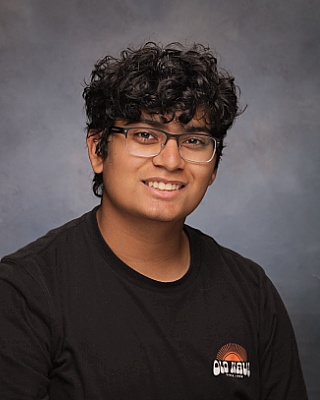
\includegraphics[width=1in,height=1.25in,clip,keepaspectratio]{akumar.jpeg}}]{Aadarsh Kumar} is a senior in the Science and Engineering Magnet Program at Manalapan High School. His current senior project is to create a micromouse capable of mapping and navigating a maze at high speed. He is a fabulous tenor saxophonist. 
\end{IEEEbiography}
\begin{IEEEbiography}[{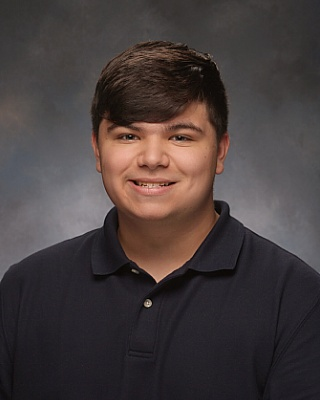
\includegraphics[width=1in,height=1.25in,clip,keepaspectratio]{sperkins.jpeg}}]{Steven Perkins} is a senior in the Science and Engineering Magnet Program at Manalapan High School. He is also an intern in the Mechanical, Electrical, and Plumbing (MEP)  division at T\&M Engineering in Middletown, NJ.
\end{IEEEbiography}
\begin{IEEEbiography}[{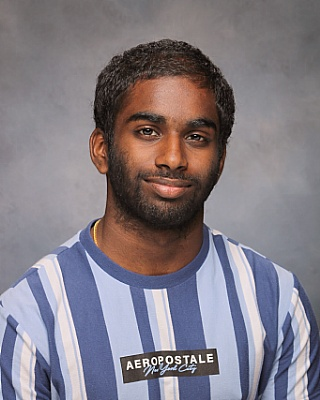
\includegraphics[width=1in,height=1.25in,clip,keepaspectratio]{nmuthukumar.jpeg}}]{Nareshsanjay Muthukumar} is a senior in the Science and Engineering Magnet Program at Manalapan High School. His current senior project is to develop a device for degassing engine coolant using ultrasound. 
\end{IEEEbiography}
\vfill
\newpage
\begin{IEEEbiography}[{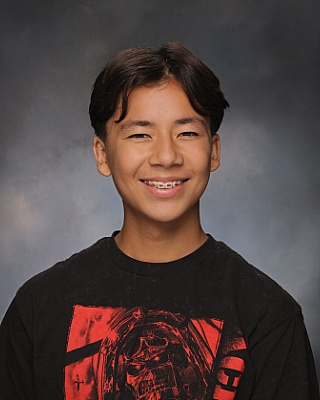
\includegraphics[width=1in,height=1.25in,clip,keepaspectratio]{hvillasenor.jpeg}}]{Henry Villase\~{n}or} is a senior in the Science and Engineering Magnet Program at Manalapan High School. His current senior project is to create a micromouse capable of mapping and navigating a maze at high speed. He is known for baking linzer torte. 
\end{IEEEbiography}
\begin{IEEEbiography}[{
\includegraphics[width=1in,height=1.25in,clip,keepaspectratio]{akhanna.jpeg}}]{Anirudh Khanna}  is a senior in the Science and Engineering Magnet Program at Manalapan High School. His current senior project is to develop a device for degassing engine coolant using ultrasound. 
\end{IEEEbiography}
\vfill

\end{document}